\section{Experimental Results}


\subsection{Roadmap}
Our experiments try to answer the following questions:

\begin{itemize}
\item bla
\item bla2
\item bla3
\end{itemize}




\subsection{Compare to Oracle}


\subsection{Analysis}
The bar-plot in Figure~\ref{fig:analy_quan} and Figure~\ref{fig:analy_prun}
shows the difference before and after using two compress techiniques respectively.


\cparagraph{Model size.}
Figure ~\ref{fig:analy_quan} a
compares the ten model size before and after using the \quantization.
As we can see from this figure, the Inception\_v1 model is
compressed from 26.1 MB to 6.8MB, which 
owns the largest compression radio, with 27.1\%.
On average, the \quantization reduces the model size by 74.5\%, 
as the relative sparse index is encoded with 8 bits, resulting in 
xxx compression in total.




\cparagraph{Energy consumption.}
Energy consumption is dominated by memory access

\begin{figure*}[!t]
\centering
\subfloat[][Model size]{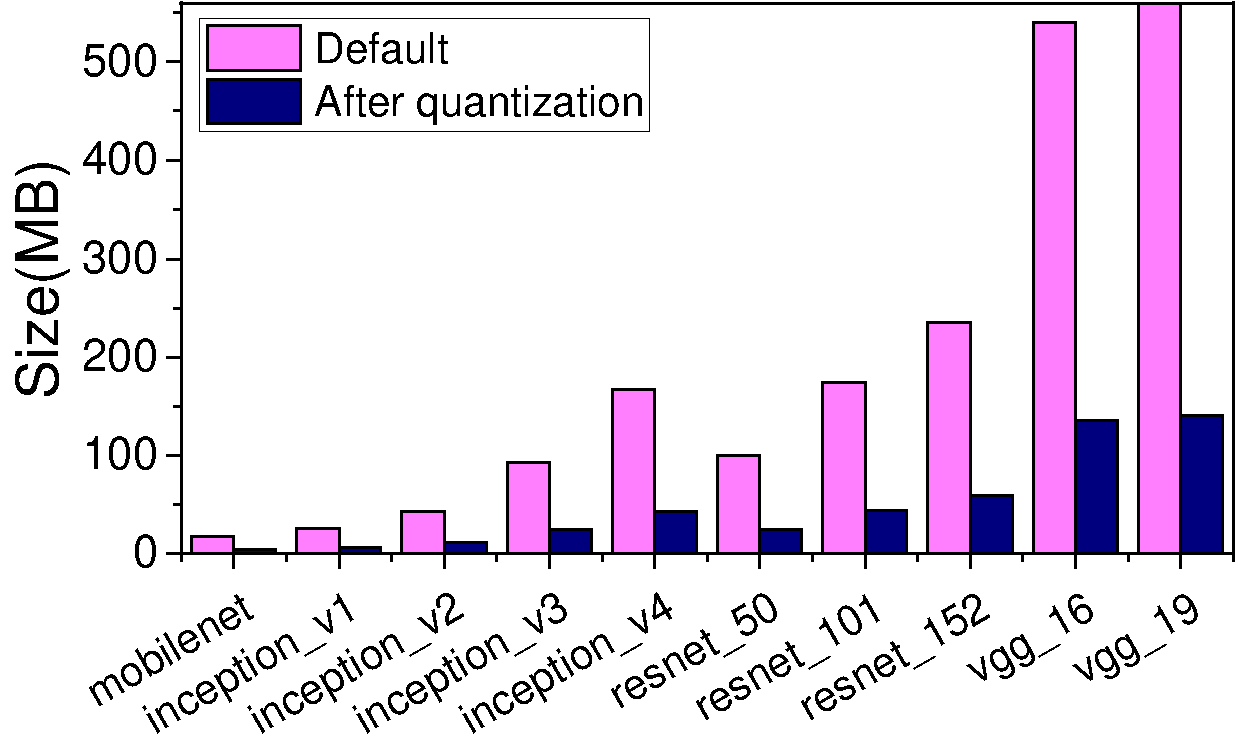
\includegraphics[width=0.3\textwidth]{figure/quan_size.pdf}}
\hfill
\subfloat[][Inference time]{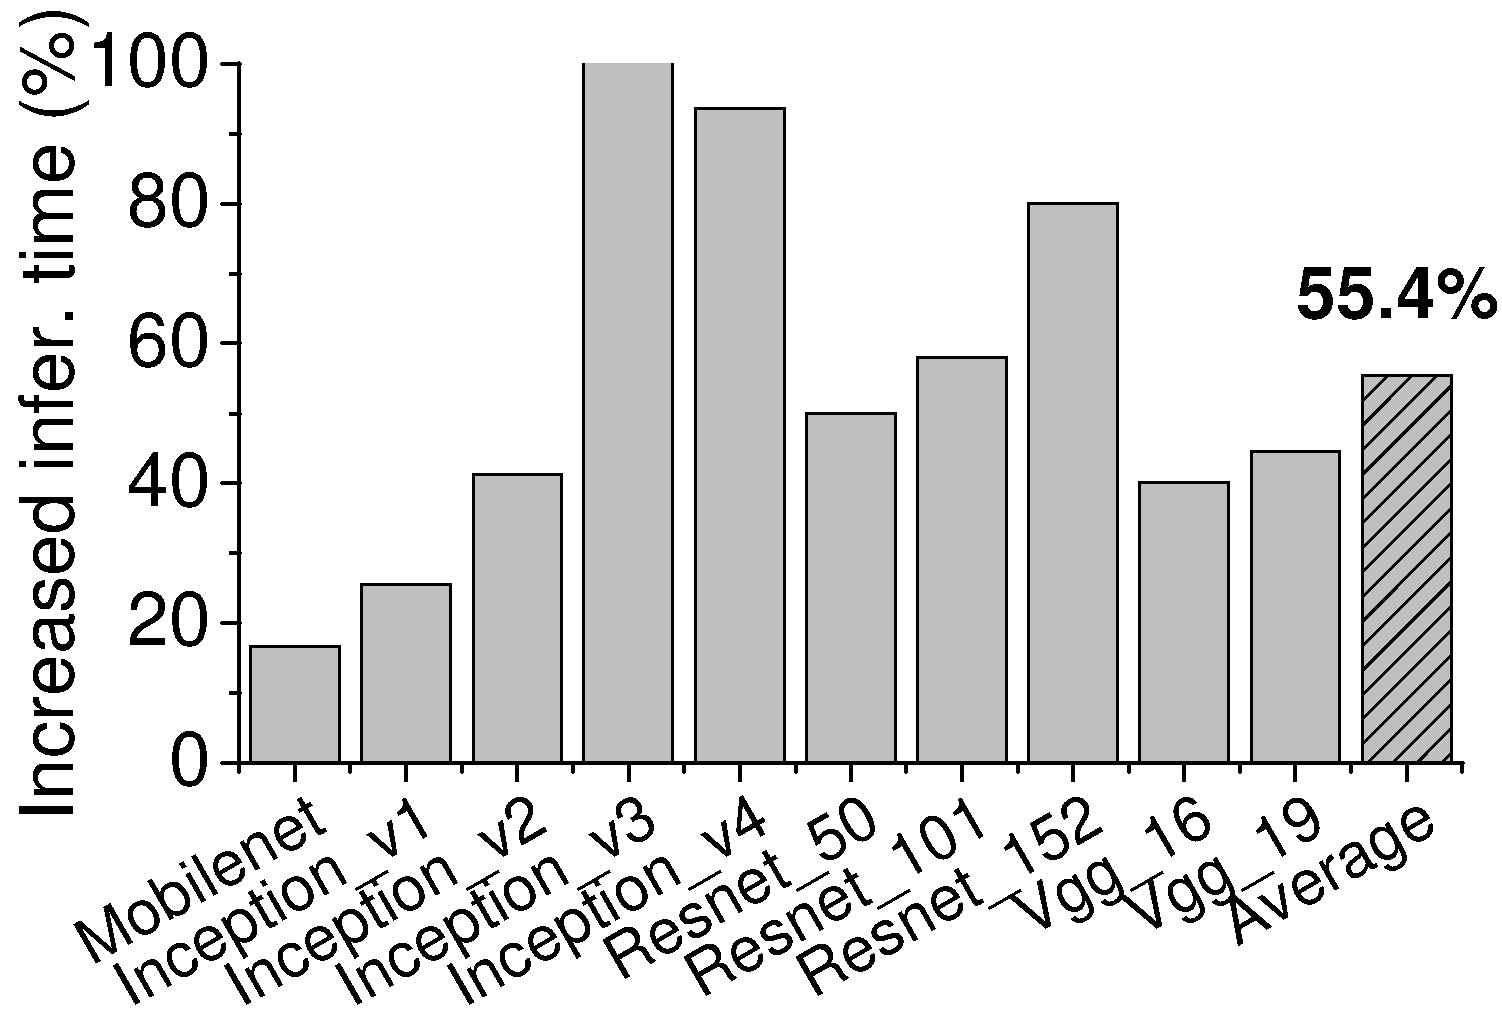
\includegraphics[width=0.3\textwidth]{figure/quan_time.pdf}}
\hfill
\subfloat[][Accuracy]{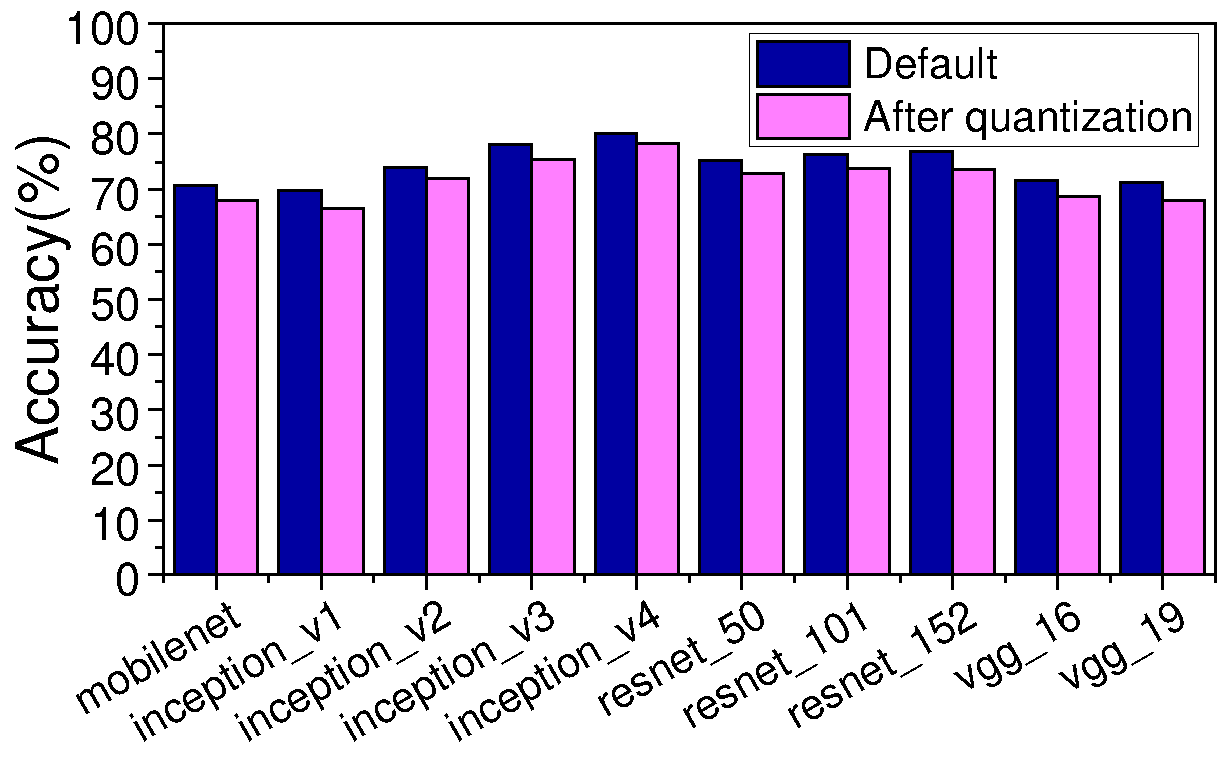
\includegraphics[width=0.3\textwidth]{figure/quan_acc.pdf}}
\hfill
\subfloat[][Power consumption]{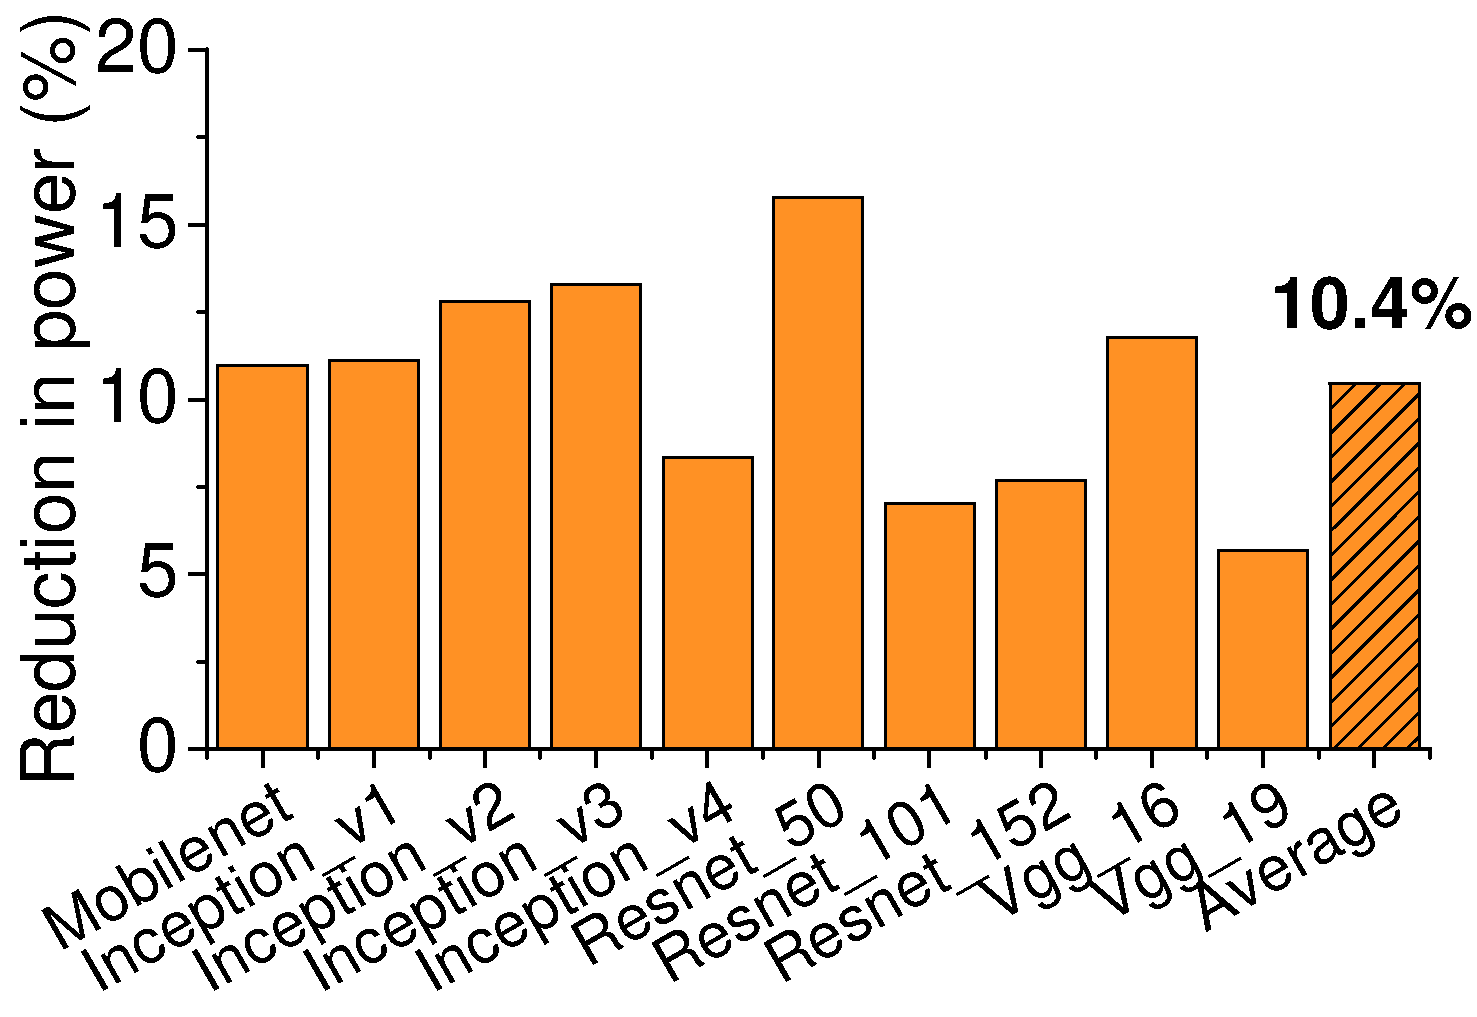
\includegraphics[width=0.3\textwidth]{figure/quan_power.pdf}}
\hfill
\subfloat[][Energy consumption]{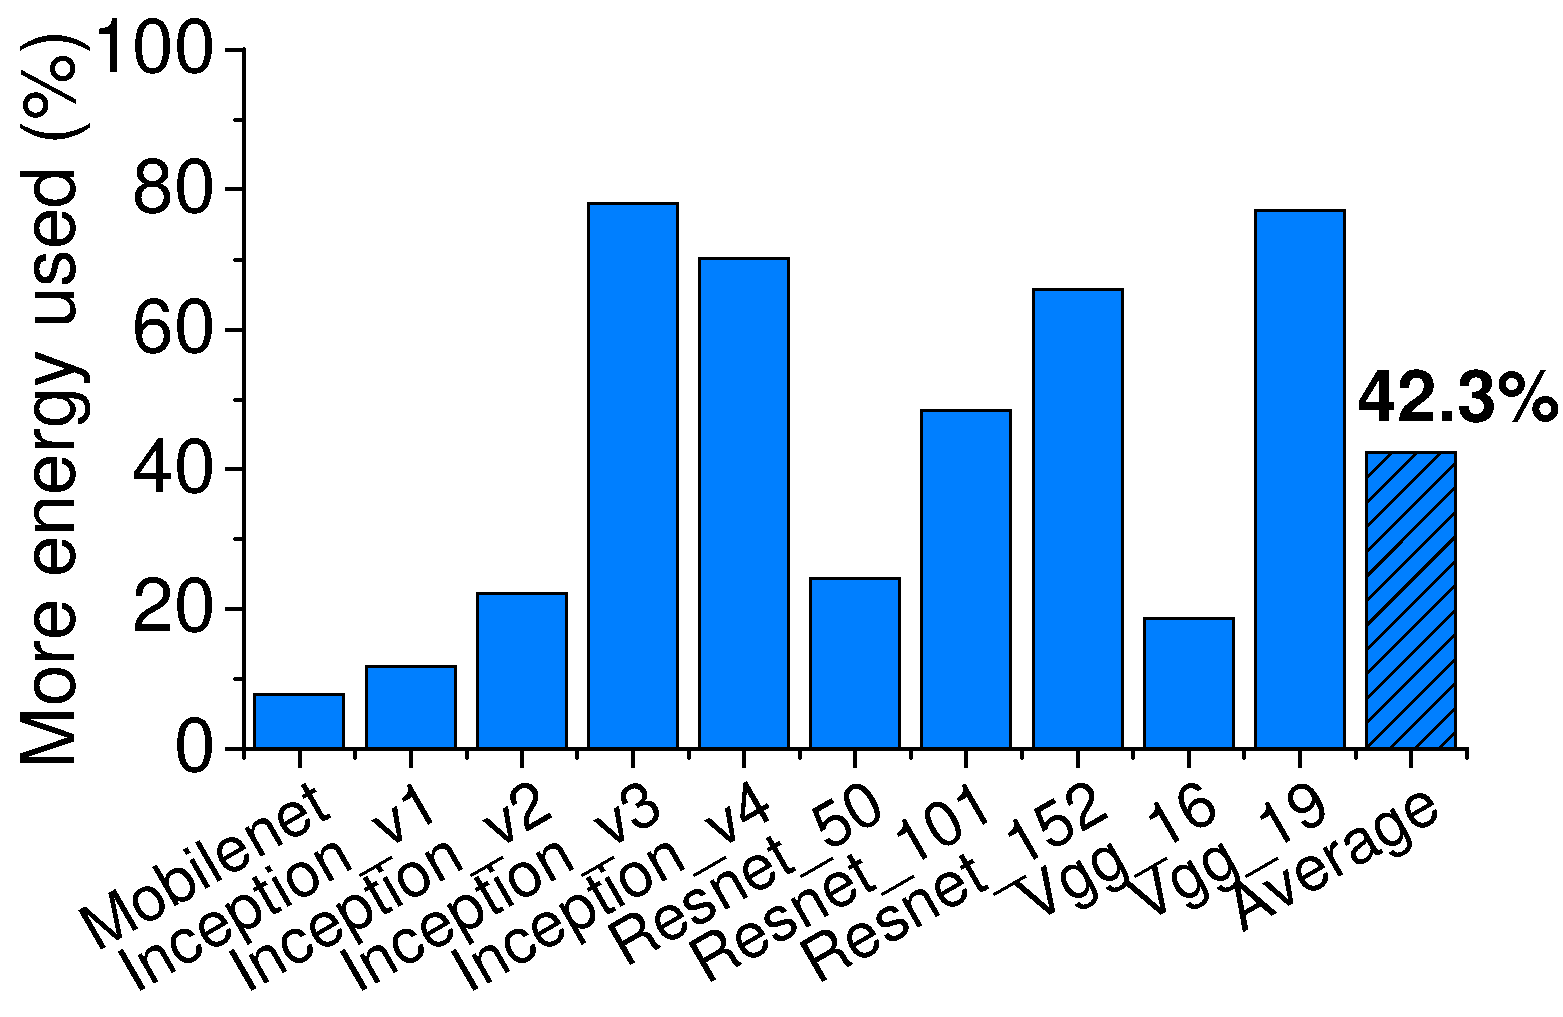
\includegraphics[width=0.3\textwidth]{figure/quan_energy.pdf}}
\hfill

\caption{The achieved model size (a) inference time (b) accuracy (c) power consumption (d) 
energy consumption (e) and F1 score (e) before and after the compression by \quantization.
The compression technique to use depends on the optimization target.\FIXME{f1 score later}}
\label{fig:analy_quan}
\end{figure*}


\begin{figure*}[!t]
\centering
\subfloat[][Model size]{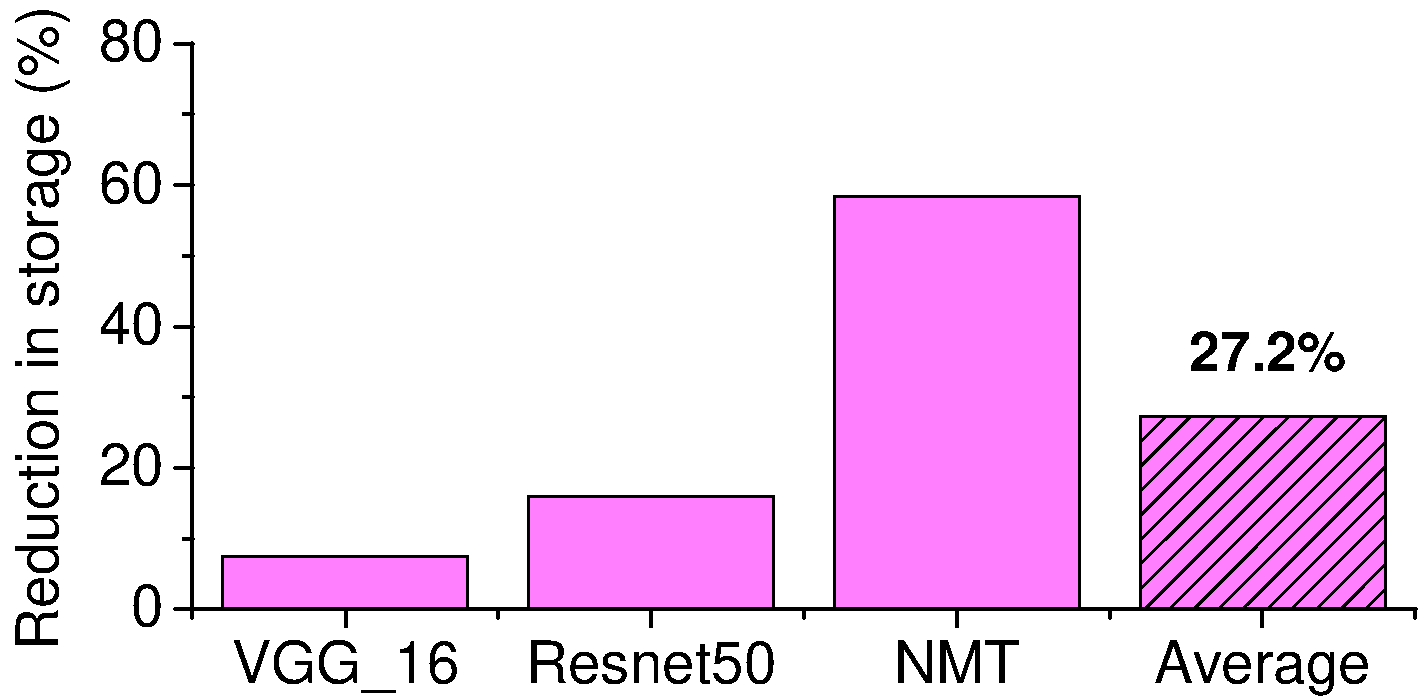
\includegraphics[width=0.3\textwidth]{figure/prun_size.pdf}}
\hfill
\subfloat[][Inference time]{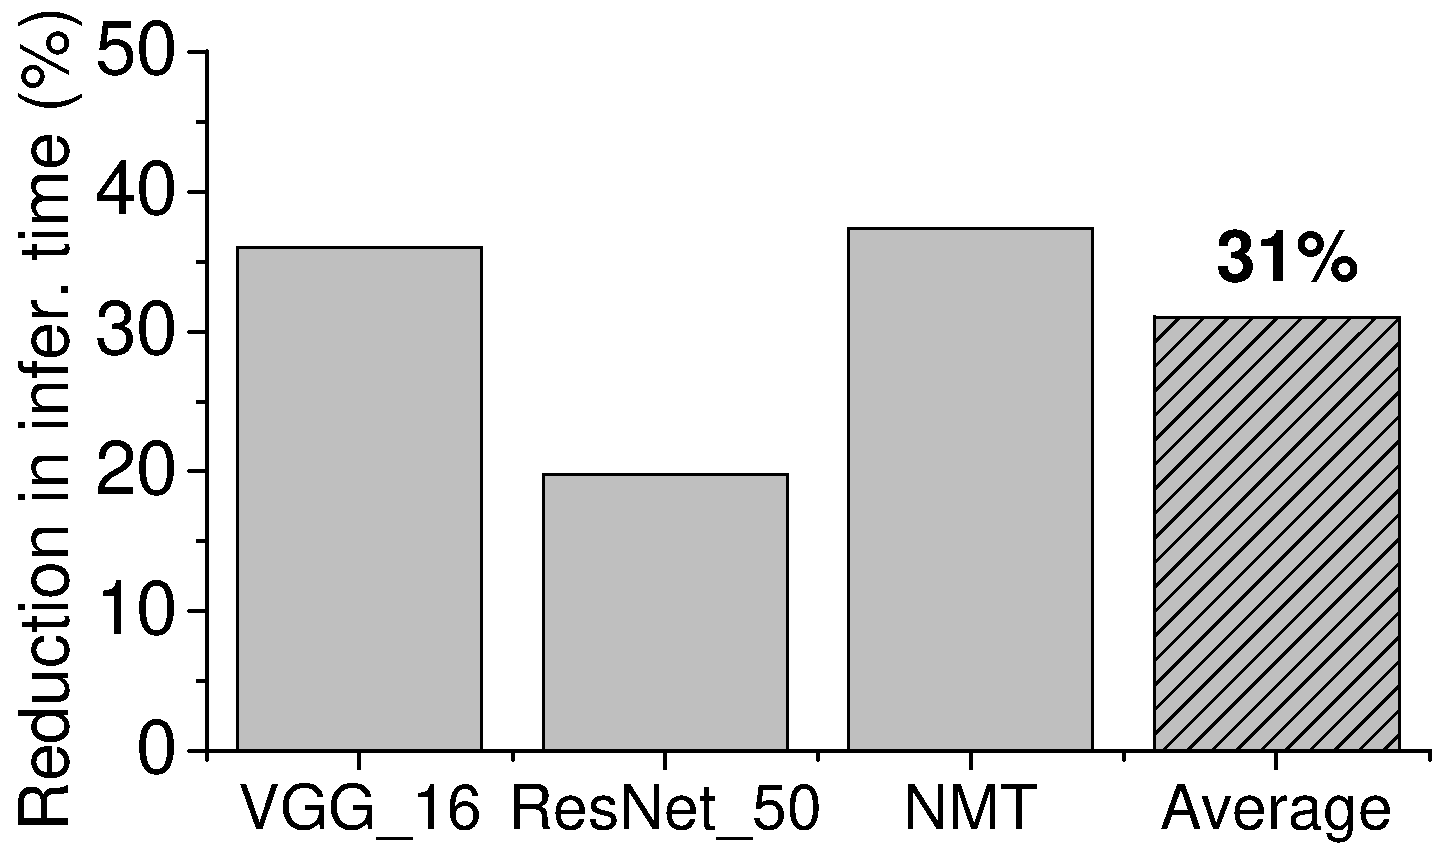
\includegraphics[width=0.3\textwidth]{figure/prun_time.pdf}}
\hfill
\subfloat[][Accuracy]{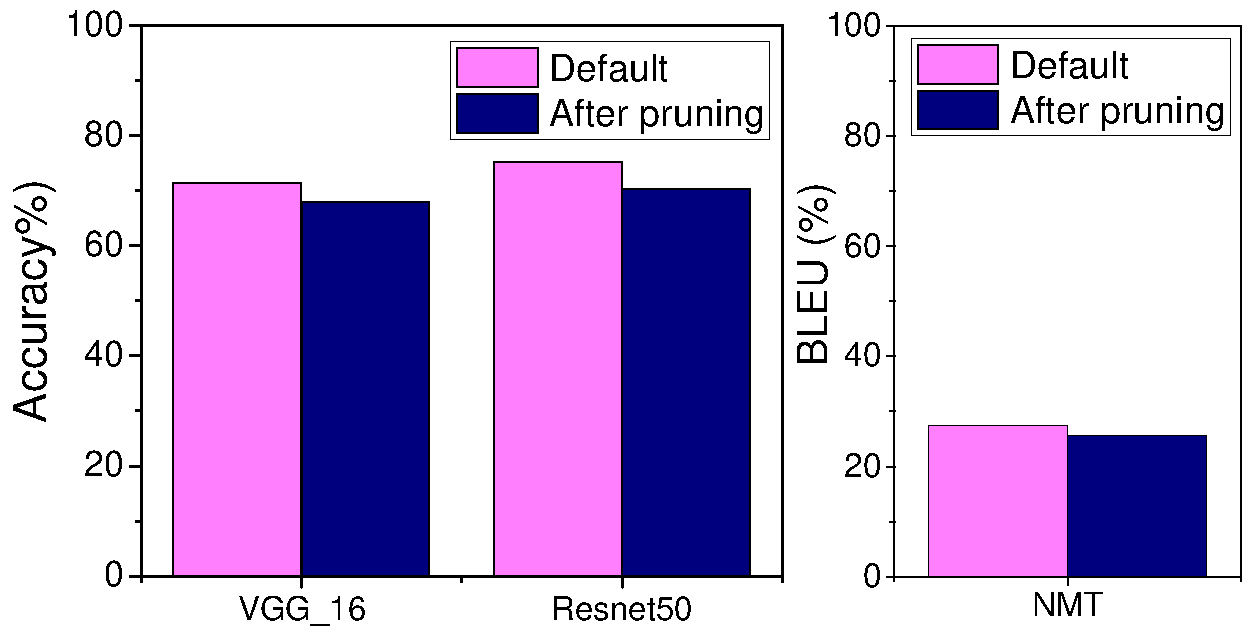
\includegraphics[width=0.3\textwidth]{figure/prun_acc.pdf}}
\hfill
\subfloat[][Power consumption]{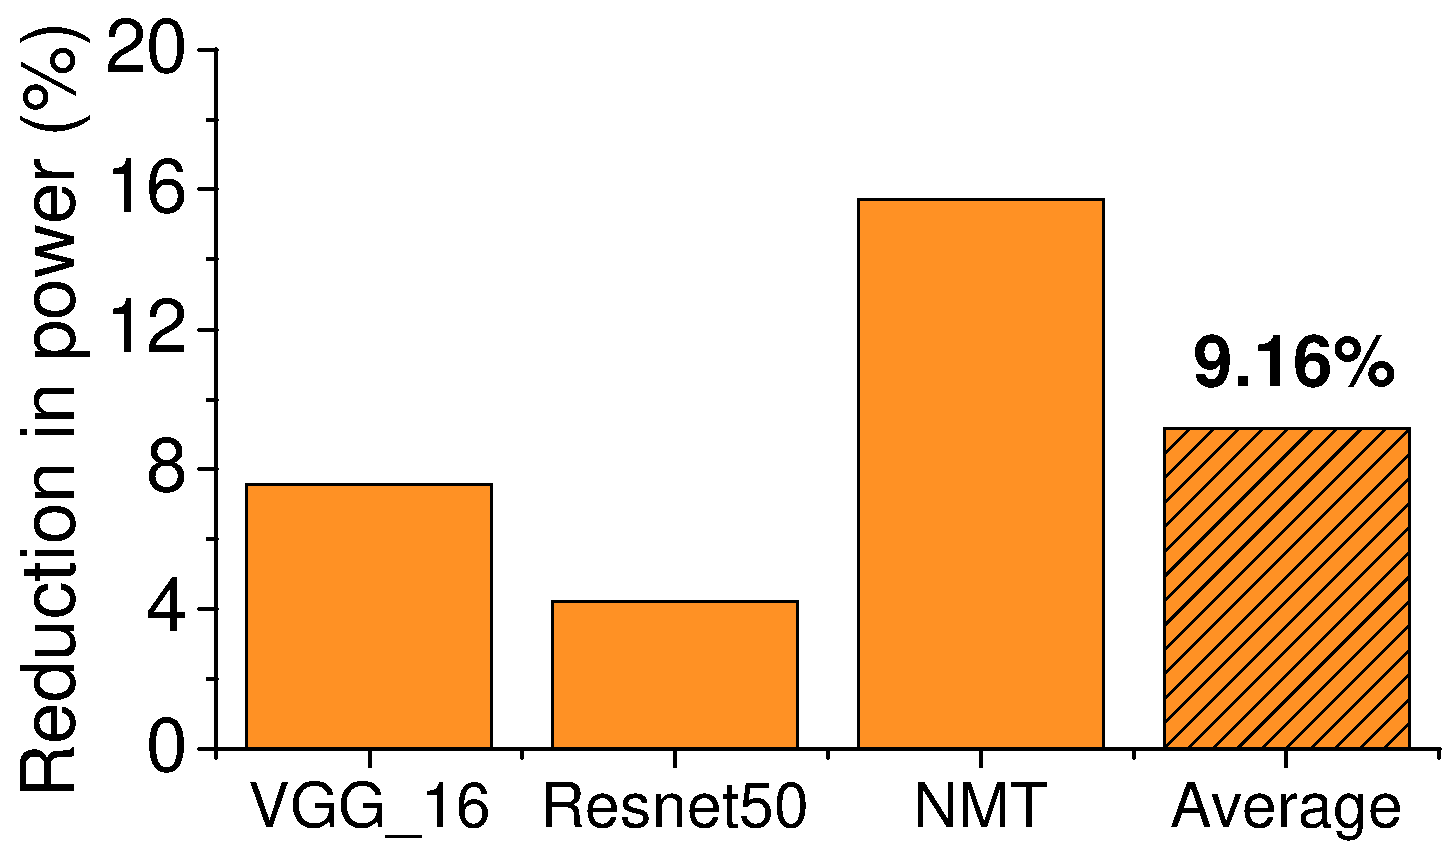
\includegraphics[width=0.3\textwidth]{figure/prun_power.pdf}}
\hfill
\subfloat[][Energy consumption]{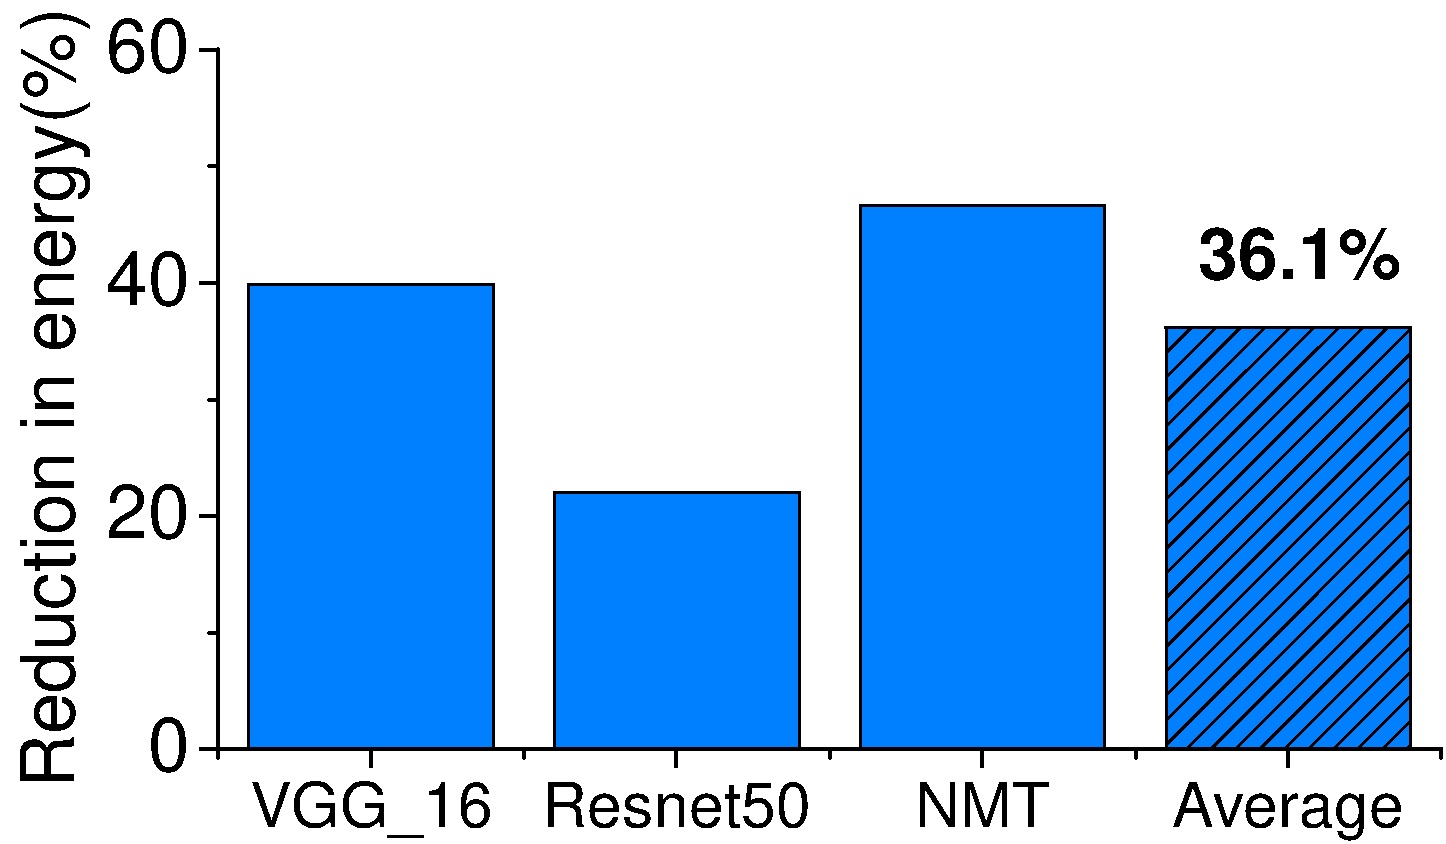
\includegraphics[width=0.3\textwidth]{figure/prun_energy.pdf}}
\hfill

\caption{The achieved model size (a) inference time (b) accuracy/BLEU (c) power consumption (d) 
energy consumption (e) and F1 score (e) before and after the compression by \pruning.
The compression technique to use depends on the optimization target.\FIXME{f1 score later}}
\label{fig:analy_prun}
\end{figure*}